% !TEX TS-program = pdflatex


\section{Summary}
% Context
Leveraging the time-honored principles of modularity and 
reuse, modern software 
systems development typically entails the use of external 
libraries.
Rather than implementing new systems from scratch, developers 
look for, and try 
to integrate into their projects, libraries that provide 
functionalities of 
interest. Libraries expose their functionality through 
Application Programming 
Interfaces (APIs) which govern the interaction between a 
client project and the 
libraries it uses.

% Learning APIs
Developers therefore often face the need to learn new APIs.
The knowledge needed to manipulate an API can be extracted 
from various 
sources:~the API source code itself, the official website and 
documentation, 
Q\&A websites such as StackOverflow, forums and mailing 
lists, bug trackers, 
other projects using the same API, etc.
However, an official documentation often merely reports the 
API description 
without providing non-trivial example usages. Besides, 
querying informal 
sources such as StackOverflow might become time-consuming and 
error-prone~\cite{robillard2009makes}.
Also, API documentation may be ambiguous, incomplete, or 
erroneous~\cite{uddin2015api}, while API examples found on 
Q\&A websites may be 
of poor quality~\cite{nasehi2012makes}.

% APIs, mining, existing tools, etc.
Over the past decade, the problem of API learning has 
garnered considerable 
interest from the research community.
Several techniques have been developed to automate the 
extraction of API 
\emph{usage 
patterns}~\cite{Robillard:2013:AAP:2498733.2498776} in order 
to 
reduce developers' burden when manually searching these 
sources and to provide 
them with high-quality code examples. However, these 
techniques, based on 
clustering~\cite{Niu2017API, Wang2013Mining, Zhong2009MAPO} 
or predictive 
modeling~\cite{Fowkes:2016:PPA:2950290.2950319}, still suffer 
from high 
redundancy~\cite{Fowkes:2016:PPA:2950290.2950319} and---as we 
show later in the 
thesis---poor run-time performance.

To cope with these limitations, a new approach is proposed in 
this thesis to 
recommend to developers items that have been bought by 
similar users in similar 
contexts. Informally, the question the proposed system can 
answer is:

\begin{quote}
	\textit{``Which API methods should this piece of client 
	code invoke, 
	considering that it has already invoked these other API 
	methods?"}
\end{quote}
%We transpose this idea in the context of API 
%recommendation:~should the method 
%currently being written (a customer) invoke (buy) a method 
%from an API (a 
%product) given the context of the current project?

%%%%%%%%%%%%%%%%%%%%%%

A real big issue is how to perform a good enough 
recommendation in this 
context, balancing possible bias and putting the proper hints 
for the 
developer. Moreover, the form of the recommendation is also 
important because, 
in general, there are variety of possible suggestion such as 
code snippet, 
patterns for the methods, enhance documentation and all 
things that make a 
recommendation really usable for the current project. 

This work is developed within the European H2020 CROSSMINER 
project~\cite{CROSSMINER} that aims at conceiving techniques 
and tools for developing new software systems by reusing 
existing open source 
components. Nowadays, the complex software system are really 
big and it is not 
so easy to select and deploy a component in the right way. 
The planned 
CROSSMINER technical offering consists of the following 
analysis tools:

\begin{itemize}
	\item \textit{Source code analysis tools} to extract and 
	store knowledge from the 	source code of a collection of 
	open-source projects;
	\item \textit{Natural language analysis tools} to extract 
	quality metrics related to 	the communication channels, 
	and bug tracking systems of OSS projects by using Natural 
	Language Processing and text mining techniques;
	\item \textit{System configuration analysis tools} to 
	collect and analyse system 	configuration artefacts;
	\item \textit{Workflow-based knowledge extractors} that 
	simplify the analysis of a complex software system;
	\item \textit{Cross-project relationship analysis tools} 
	to manage a wider range of open source project 
	relationships, such as dependencies and conflicts, 
	based on user-defined similarity measures and the 
	creation of project clusters;
	\item \textit{Advanced integrated development 
	environments} that will allow developers to adopt the  
	knowledge base and analysis tools directly from the 
	development environment, that providing alerts, 
	recommendations, and user feedback which will help 
	developers to improve their productivity.
\end{itemize}

Figure \ref{fig:crossminerApproach} shows an overview of the 
CROSSMINER 
approach at work. In such a context, the work presented in 
this thesis wants to 
propose a novel tool that perform API function call 
recommendations in the 
context of Java projects. It is integrated in the CROSSMINER 
knowledge base 
component in a  flexible way. 



\begin{figure}[!t]
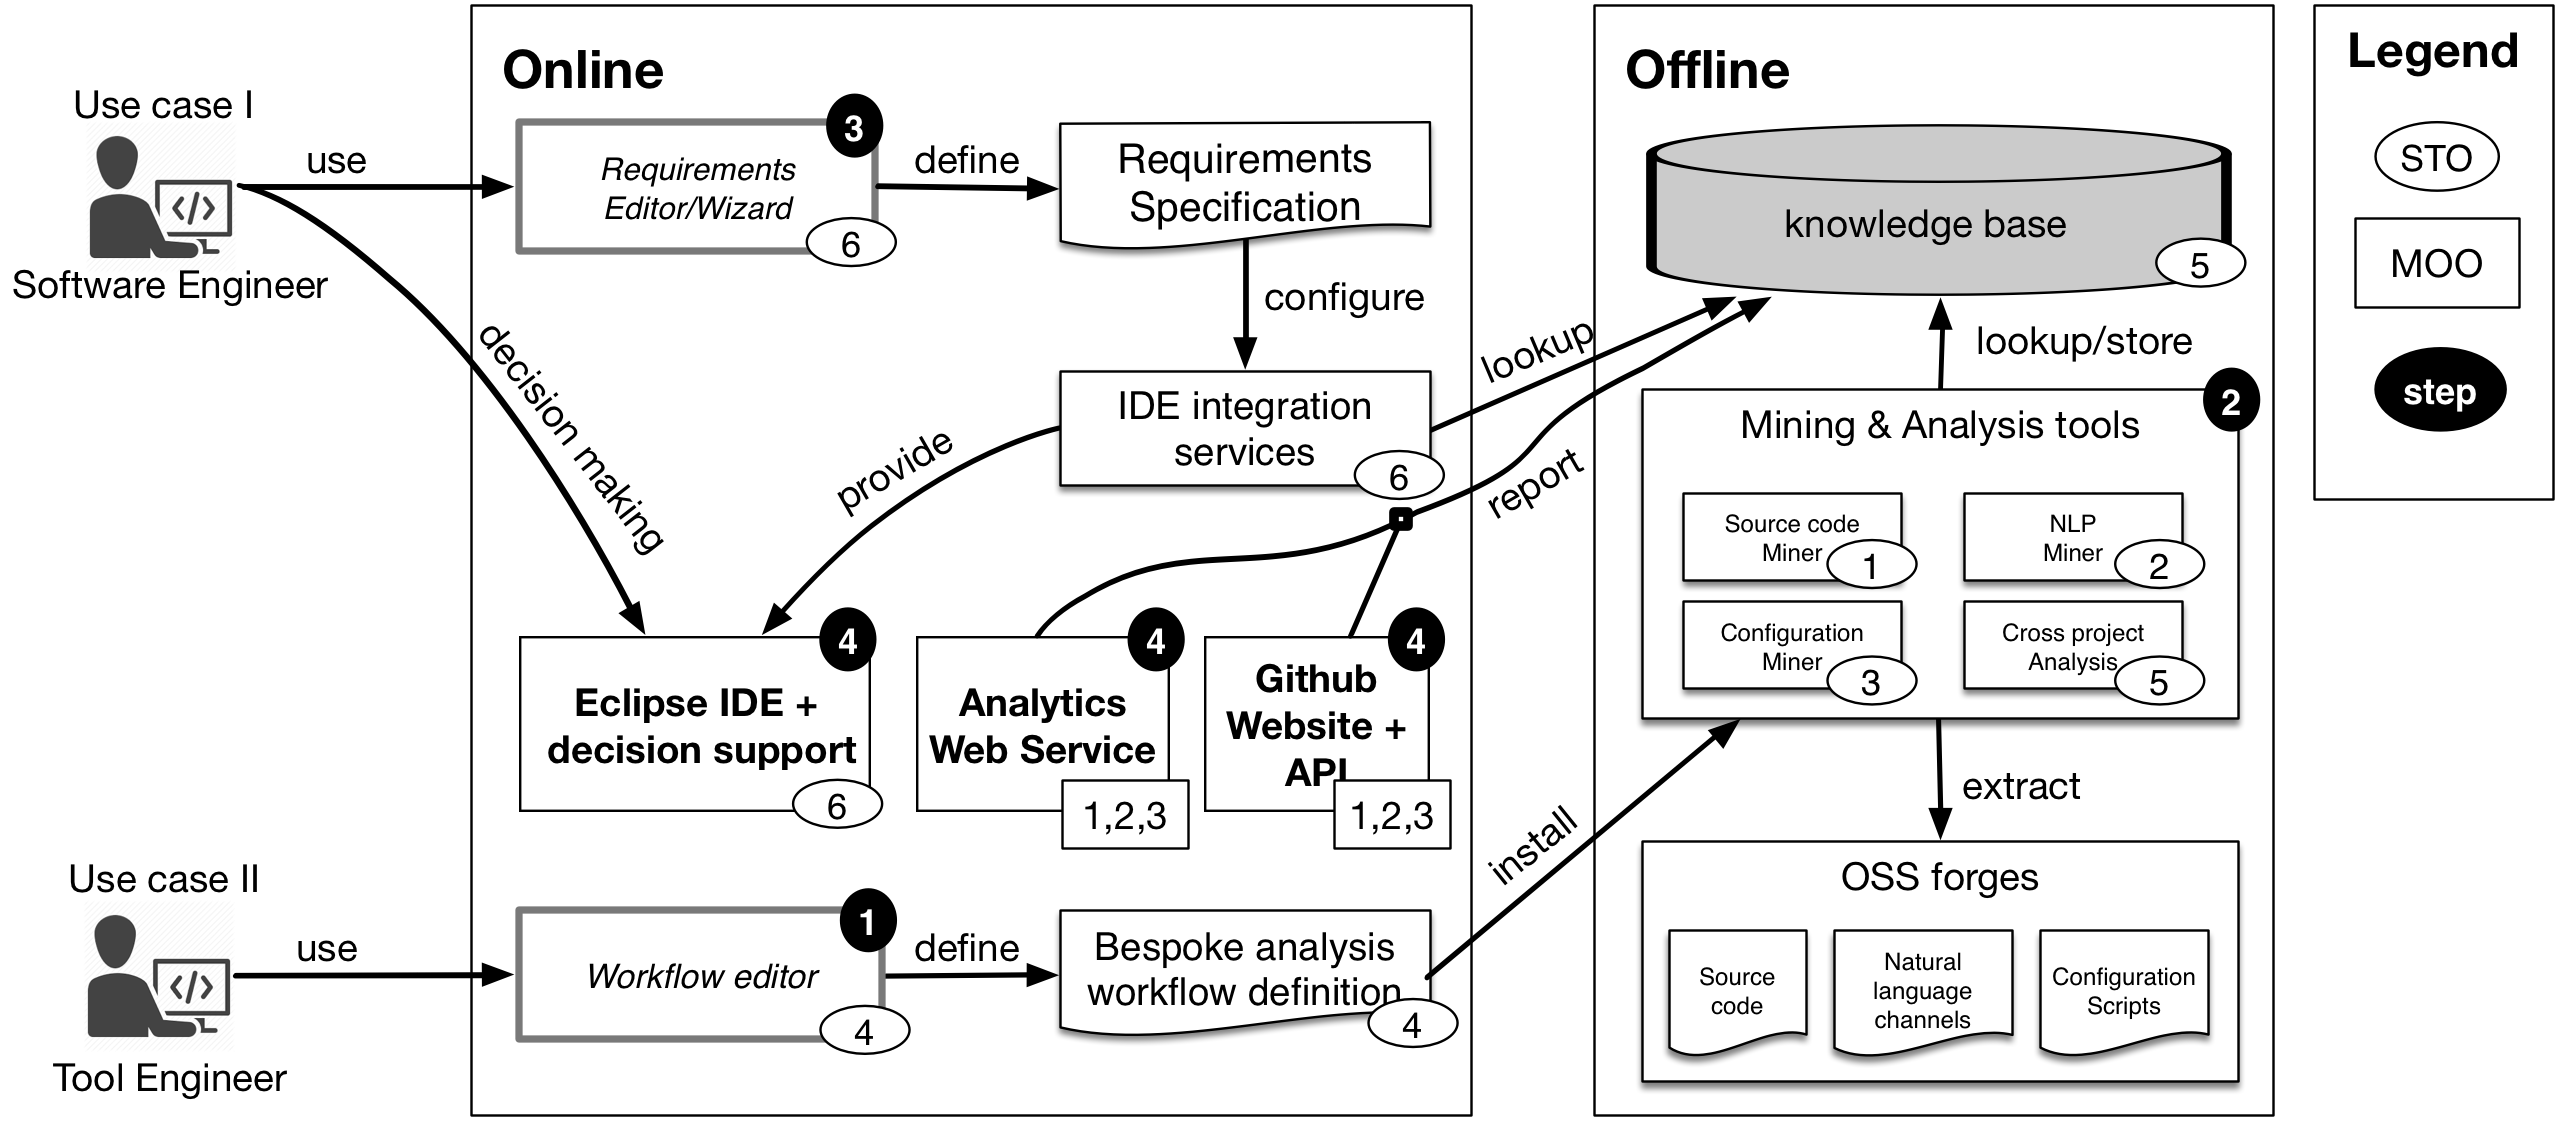
\includegraphics[width=14cm,height=14cm,keepaspectratio]{images/crossminer.png}
\centering
\caption{The CROSSMINER project at work}
\label{fig:crossminerApproach}
\end{figure}


\section{Research Objectives}
\begin{figure}[!h]
	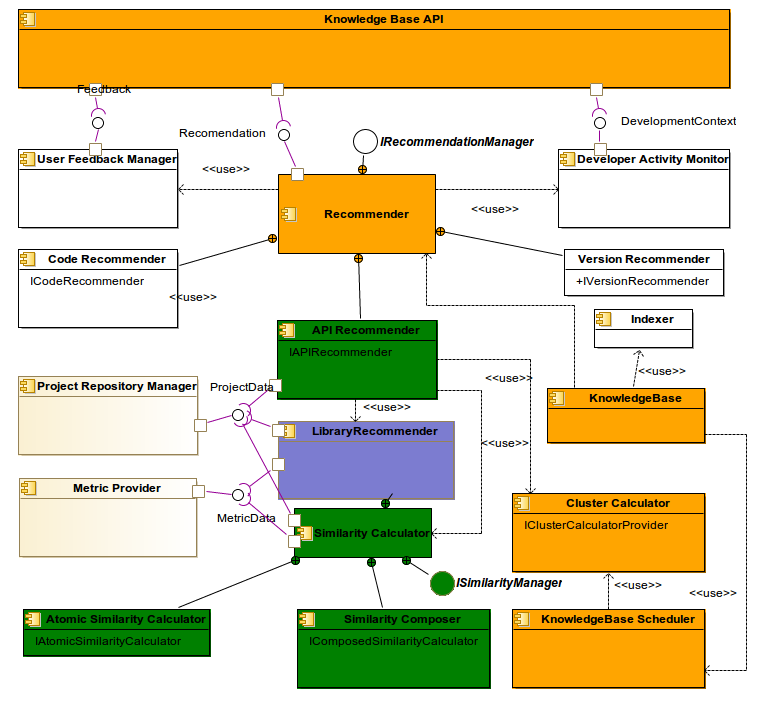
\includegraphics[width=12cm,height=12cm,keepaspectratio]{images/Kb.png}
	\centering
	\caption{An overview of the CROSSMINER knowledge base}
	\label{fig:crossminerKB}
\end{figure}

Figure \ref{fig:crossminerKB} shows an overview of the 
CROSSMINER 
knowledge base underpinning the whole recommendation 
mechanism; the proposed 
approach gives support for the \code{APIrecommender} 
subcomponent in the 
picture. In particular, we combine the concepts of code 
cloning and patterns to 
retrieve real code snippets that show a concrete usage of the 
libraries used by 
the developer. We choose this approach because code snippets 
represent 
immediate hints in the developing context, as a concrete 
usage of a method or 
class is more relevant rather than a JavaDocumentation 
description or the list 
of imports. We exploit also the code cloning technique in 
order to search and 
retrieve possible suggestion.

\section{Thesis Structure}

The thesis is organized in the following chapters:

\begin{itemize}
	\item Chapter 2 introduces the context of this thesis. 
	The notions of 
	recommendation systems and API mining are introduced. 
	Code cloning 
	techniques are also overviewed as underpinning the API 
	recommendation 
	approach proposed in Chapter 4 of this thesis.
		
%	In particular provides a general overview on the key 
%concepts used in the 
%	developed of the proposed tool. These concepts are the 
%definition of API 
%	and recommendation; there are very general terms and the 
%literature are 
%	plenty of examples and definitions in such a way that it 
%is impossible to 
%	give an exhaustive overview. For this reason, we try to 
%define in the right 
%	manner the context suitable for the proposed approach, by 
%avoiding the 
%	perfect coverage of the topic and limit ourself to a few 
%but relevant 
%	concepts for our aims. Moreover, we provide a general 
%state of the art of 
%	the code cloning domain, with some definitions as cloned 
%fragment, sources 
%	units and comparison algorithms. We also present 
%different code cloner to 
%	have an overview on the different approaches and finally, 
%we present 
%	Simian, the code cloner used in the proposed approach.
	
	\item Chapter 3 presents an overview of existing 
	approaches able to mine 
	APIs. A comparative table is presented at the end of the 
	chapter with 
	respect to peculiar features.
	
%	Section 3 gives an overall view of the problem, 
%considering the most 
%	used and famous tool used for facing the API 
%recommendation problems. They 
%	use very different techniques and a state of the art is 
%necessary to better 
%	understand approaches, level of the recommendations and 
%possible issues 
%	that arise when we develop these kind of systems.The 
%general API 
%	recommendations procedure involves the visit of the AST, 
%some clustering 
%	techniques and a ranking as postprocessing phase and we 
%compare various 
%	existing approaches. Among these works, we select CLAMS 
%for its results to 
%	perform our recommendations and PAM  for validate our 
%approach. 
	
	\item Chapter 4 presents the proposed approach, which 
	relies on the combined
	adoption of the existing CLAMS and Simian tools presented 
	in Chapter 3. In 
	particular, CLAMs is used to create snippets of code 
	representing recurring 
	patterns in the analyzed APIs. Subsequently, Simian is 
	used to analyze the 
	developer's context, that contains what she is developing 
	and, in 
	particular, the fragment of code on which she would like 
	to get 
	recommendations. As final outcome, the proposed approach 
	is able to provide 
	developers with novel patterns in the form of snippets of 
	code that 
	contains method invocation and all the variables that are 
	needed to execute 
	them in the proper way.
	
	\item Chapter 5 presents an evaluation of the proposed 
	recommendation 
	approach.
	%In the Section 5, we propose an evaluation framework 
	%based on AST of  the 
	%code.The aim of this framework is to validate in an 
	%empirical way the 	
	%produced recommendations by analysing the method 
	%declarations and 	
	%invocations. To do this, we use JavaParser to retrieve 
	%the snippet of 
	%code 	
	%that represent the context and Rascal, a meta 
	%programming language, to 	
	%parse the AST of the developer's project in order to 
	%represent in the 	
	%proper way the context, very important to evaluate if 
	%the suggested 	
	%patterns are the correct ones for it. 
	The evaluation is performed by 
	considering four metrics: \textit{precision}, 
	\textit{recall}, 
	\textit{success rate} and \textit{F-measure}. 
%	All the metrics are explained in the related section and 
%it is used on the 
%	list of method invocations retrieved by Rascal. Moreover, 
%we use PAM as to 
%	compare the final results. 

	\item Chapter 6 concludes the thesis and performs an 
	analysis of possible 
	future works.
%	 in this area, starting from an improvement in the 
%	recommendation format and alternative techniques with 
%respect to the code 
%	cloning used for this work.
	
\end{itemize}

